\chapter{Theoretical Background}
\label{the}
This chapter presents the basic theories and knowledge that this thesis is built upon.

\section{Machine Translation}
\label{the-mt}

\textit{Machine translation} is an area of computational linguistics aiming to automatically translate text or speech from the \textit{source} language to the \textit{target} language.

Machine translation is distinct from computer-aided translation in which human translators use computer software to support the translation process.
Machine translation should be performed on a fully automatic basis without any human interaction. 
Obviously, a machine translation system can be used during computer-aided translation.

The two most common types of MT system are rule-based and statistical.
These types differ in the way that they are built, but are often combined within the same system which is then called \textit{hybrid MT}.

\textit{Rule-based machine translation (RBMT)} considers language as a set of rules capturing all the relevant regularities in morphology, syntax, or other layers of language description.
In order to translate a sentence, it employs a predefined set of rules within the language to break down the sentence.
Then, another set of rules links between the source and target language, and a robust bilingual dictionary is used to carry out the translation.
These rules are essential for building such a system, but they are usually expensive to construct and must be created anew for each new language pair.

On the other hand, \textit{statistical machine translation (SMT)} does not use linguistic rules to translate but instead a statistical model.
For each unit of the source sentence, there are several possible translations associated with a probability.
% Stress that linguistics *is* usually used when deciding what are the units
The goal of the SMT system is to select these translations for each source unit such that they cover the source sentence with the highest translation probability.
The statistical model helps this selection process, parameters of which must be derived from a sufficient amount of data.
The data in this case is called the \textit{bilingual corpus}, a set of pairs, each consisting of a sentence from the source language and the corresponding sentence in the target language.

From the mid 2010s, the field of MT has seen a new group of systems emerge and then outperform the two previously mentioned types to establish the new state of the art.
These MT systems are actually not too different from SMT as they are also statistical learning models.
However, they employ deep neural networks, which have been very successful in computer vision and simpler linguistic tasks, to model the translation task.
Hence, this type is referred to with a distinct name, \textit{neural machine translation}, which will be discussed in detail in the following section.

\subsection{Neural Machine Translation}
\label{the-mt-nmt}
As mentioned above, a \textit{neural machine translation} system uses a deep neural network to learn the statistical model for machine translation.
Unlike the statistical MT, where all types (word-based, phrase-based or syntax-based) consist of several sub-components that need to be trained separately, NMT can be built and trained in a single neural network.
Such a system is referred to as end-to-end, in which the model is trained at once, directly mapping an input source sentence to its associated sentence in the target language.

The use of neural networks in MT dates back to the works of \cite{Castano97machinetranslation} and \cite{neco1997asynchronous}.
After a break, NMT returned and has started to show promising results with the sequence-to-sequence (\seq2seq) model proposed by \cite{DBLP:conf/nips/SutskeverVL14}.
The idea was based on the assumption that when translating a sentence (in text or speech), a human reads or listens to the whole sentence, understands it, then starts to write down the translated sentence token by token.
Therefore, \seq2seq consists of two main components: an \textit{encoder} and a \textit{decoder} (\cref{fig:seq2seq}).
The encoder consumes the source sentence and produces a fixed-length vector encoding the ``meaning" of the sentence.
This vector is then fed to the decoder.
Finally, the decoder produces the target sentence in the target language token-by-token, based on the context vector and the previously translated tokens. 
In the \seq2seq model, the encoder and decoder are both modelled by a recurrent neural network, or its variant, \textit{long-short term memory} (LSTM) \citep{Hochreiter95longshort-term}.

\begin{figure}
    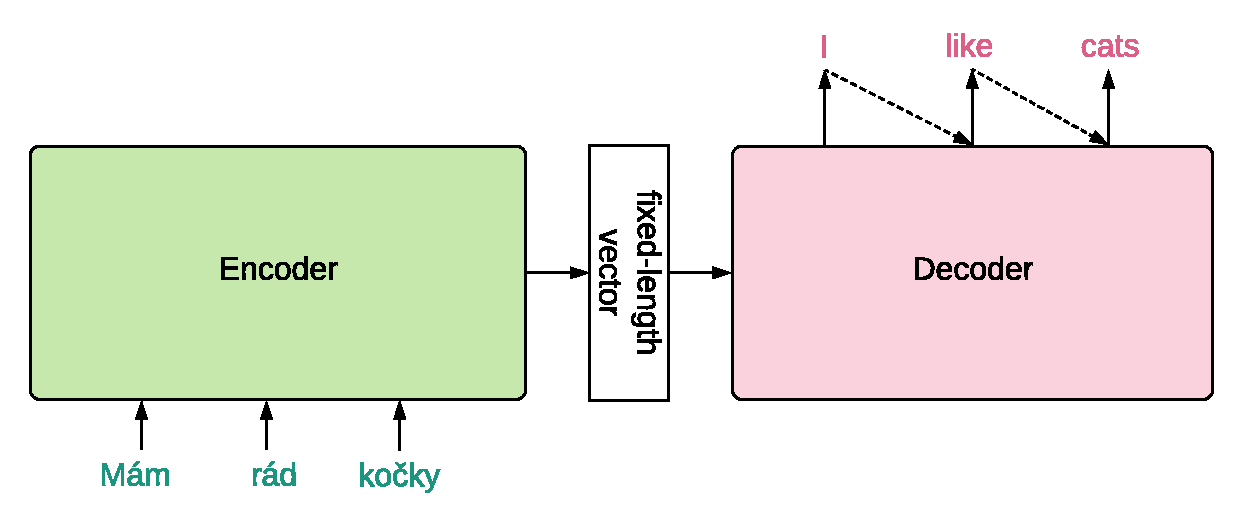
\includegraphics[width=\linewidth]{img/seq2seq.pdf}
    \caption{\seq2seq model.}
    \label{fig:seq2seq}
\end{figure}

\subsection{Attention Mechanism}
\label{the-mt-att}
The assumption that human translators keep in mind the meaning of the entire source sentence is arguable.
Some might argue that the translator has to look back to some part of the source sentence during the translation process.

We are yet to know which is the correct way our brain works during the translation process.
However, from the technical point of view, the limitation of the encoder-decoder approach is that the encoder has to output a fixed-length vector from the source sentence, which is then used in the decoder to output the target sentence.
This means that every decoded token $w$ is condition from the same vector, which captures the whole source sentence, instead of from some parts, e.g. clauses, phrases, etc., of the source sentence which are most associated with $w$.
% This means that all decoded words are based on the same context vector, sentence level instead of the part that gives the most information (clause, phrase, etc.).
In addition, compressing all information into a fixed-length vector leads to the loss of information when the sentence becomes longer.
This is where the attention mechanism is able to help \seq2seq.

\Cref{fig:seq2seq-att} illustrates this mechanism. When translating the second token, the model does not only take into account the information from $s_1$, but also looks back to the encoder. The main computational steps of the attention layer are:
\begin{itemize}
    \item Compute the \textit{attention weights} $a_{2,1}$, $a_{2,2}$, $a_{2,3}$.
    \item Compute the \textit{context vector} $c_2 = a_{2,1}h_1 + a_{2,2}h_2 + a_{2,3}h_3$.
    \item Feed $c_2$ to the computation of $s_2$.
\end{itemize}

\begin{figure}[t]
    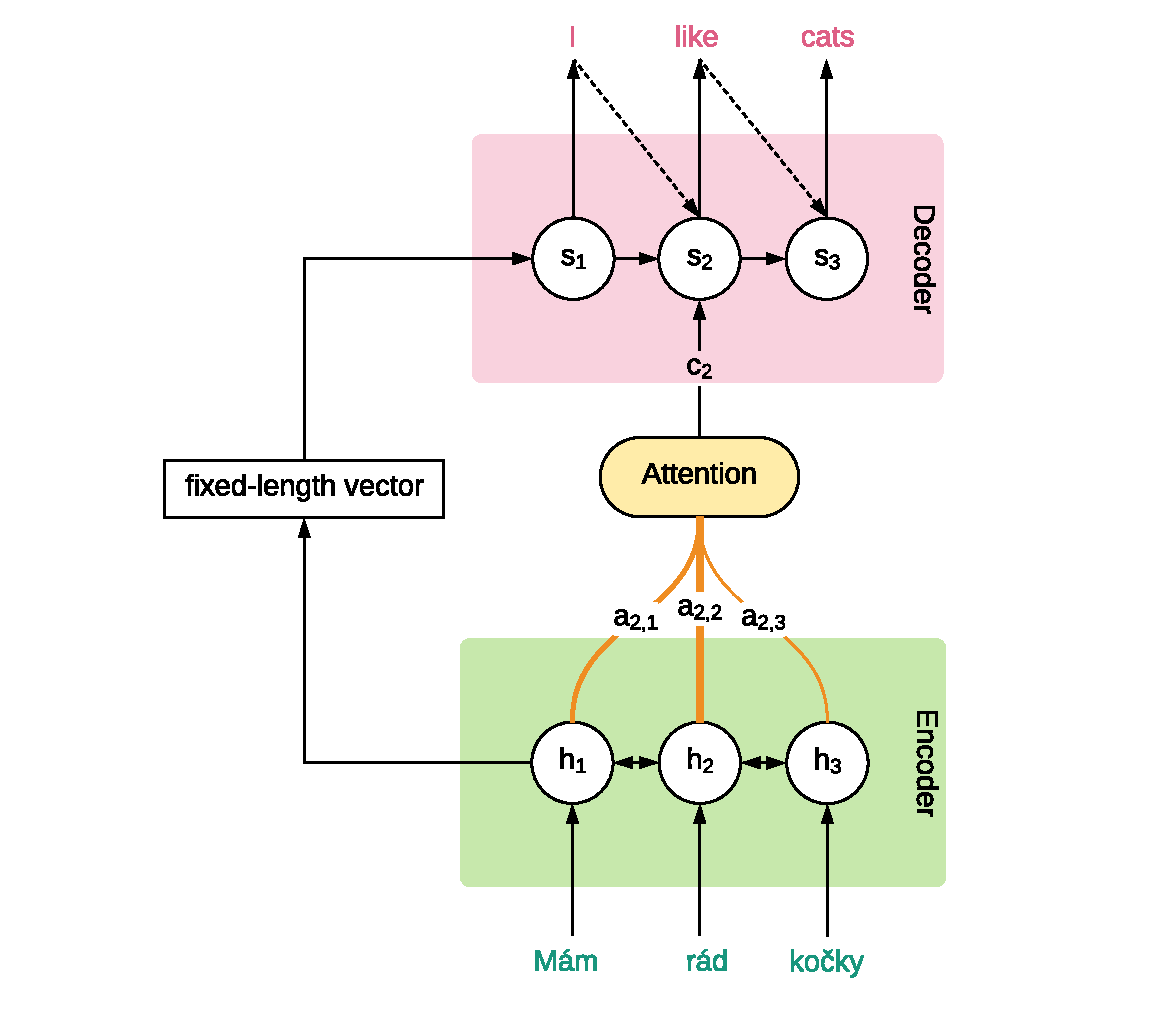
\includegraphics[width=\linewidth]{img/seq2seq-att.pdf}
    \caption{\seq2seq model with Bahdanau attention.}
    \label{fig:seq2seq-att}
\end{figure}


\cite{bahdanau:etal:attention:iclr:2015} proposed the formulas to compute the attention weight $a_{i,j}$ as follows:
\begin{enumerate}
    \item $e_{i,j}=att(s_{i-1}, h_j)$, where $e_{i,j}$ is the \textit{attention energy}, $s_{i-1}$ is the previous hidden state of the decoder, $h_j$ is the hidden state at position $j$ in the encoder.
    \item $a_{i,j}=\frac{exp(e_{i,j})}{\sum_{t}exp(e_{i,t})}$.
\end{enumerate}

The function $att$ is simply a dot product between two vectors. The second step is the \textit{sigmoid function}, ensuring that $\sum_{t}a_{i,t} = 1$, i.e. a distribution. 

This attention mechanism brings a significant improvement to the \seq2seq model.
In some examples, the attention weight matrix is visually similar to the alignment matrix from SMT.
Hence, the attention was also considered as soft-alignment because it does not need to strictly match tokens between the two sentences.

\cite{DBLP:conf/emnlp/LuongPM15} called this type of attention \textit{global attention}, to differentiate from their proposed \textit{local attention}.
In local attention, the attention layer selects one token from the source sentence, then distributes the attention weights, based on a Gaussian distribution, to all neighbors of that token within a fixed-size window.
Due to the considerations of space, we will not elaborate on the local attention, which was discussed by the authors as ``complicated to implement and train".
(see the discussion\footnote{\url{https://github.com/tensorflow/tensorflow/issues/10842\#issuecomment-372546360}} for details).

\section{Evaluation}
\label{the-eval}

In this section, we discuss several methods to evaluate MT systems, which are divided into two types: manual evaluation methods and automatic metrics.

\subsection{Manual Evaluation}
\label{the-eval-manual}
Evaluating MT systems has remained one of the most important problems in the field.
Hence, there are many proposed methods, even on how humans should judge the performance of the machine-translated text.
Most of the methods simply judge the hypotheses produced by MT systems, treating the systems as black boxes.

A very straightforward evaluation is to directly assess the adequacy and fluency of whole sentences \citep{DBLP:conf/acllaw/GrahamBMZ13}.
By adequacy, the annotator is expressing to what extent MT adequately captures the meaning of the reference sentence.
In Graham, fluency is merely used to break ties in adequacy.
Another option is to rank full sentences or constituents, i.e. parts of sentences, from several MT systems.
Yet \cite{DBLP:conf/wmt/BojarEPZ11} showed that it is problematic to interpret this manual ranking.

% Comprehension test: Blind editing+correctness check.

As an alternative, task-based methods evaluate if information from MT output is as useful as the original sentence. Nevertheless, usefulness is also a vague concept and hard to measure.
% Therefore, quiz-based evaluation aims to quantify this problem of task-based evaluation in which given machine-translated snippet, evaluator is asked to answer several questions.

% HMEANT: Is the core event structure preserved? HUME
% Gray-box: Analyzing errors in systems’ output.
% Glass-box: System-dependent: Does this component work?

Although several manual evaluation methods introduced various strategies to overcome the subjectiveness of human judges, this type of evaluation is generally expensive in terms of both time and money.

% One main reason is that the evaluation is not reproducible. 
% Perhaps an even bigger problem is that the evaluation is not reproducible at a small scale.
% • Subjective (some judges are more careful/better at guessing).
% • Not quite consistent judgments from different people.
% • Not quite consistent judgments from a single person!
% • Not reproducible (too easy to solve a task for the second time).
% • Experiment design is critical!

\subsection{Automatic Metrics}
\label{the-eval-auto}

Given the problems of manual evaluation methods described above, it is natural to try to find a fast, cheap, deterministic and replicable metric. Moreover, it would be a plus if the metric allowed automatic model optimization.  

With these properties, the proposed metric can be used to check progress, allow researchers to iterate and evaluate their proposals faster and speed up the development of the field.

The \textit{BLEU} metric (Bilingual Evaluation Understudy, \cite{BLEU}) is one of these automatic evaluation metrics, which is widely used in the field of MT.
It evaluates an output (sentence or corpus) of an MT system (the candidate) by comparing it with correct translations (the references).

The two main factors of BLEU are the n-grams precisions and length of the candidate.
Precision is very commonly used in the machine learning field.
In the case of BLEU, it measures the percentage of correct n-grams in the candidate.
The trivial case is unigram ($n=1$) precision which is merely the ratio of the number of tokens shared between candidate and reference divided by the number of tokens in the candidate.
However, this simple definition of precision would not be very precise in some cases, for example:

\bigskip

\textbf{Candidate}: That \underline{that} \underline{that}

\textbf{Reference}: I think \underline{that} it is not \underline{that} bad

\bigskip

The unigram precision of the above example is 1.0 (100\%), even though only two \textit{that} unigrams in the candidate are matched with the two unigrams in the reference.
That is to say, the number of n-grams shared between candidate and reference should be clipped.
The value to use for clipping is the number of n-grams that appear in the reference. 
Having that modification, the \textit{modified n-gram precision} in BLEU is computed as follows:

\[ p_n=\frac{\sum_{C\in\{Candidates\}}\sum_{n-gram\in C}Count_{clip}(n-gram)}{\sum_{C'\in\{Candidates\}}\sum_{n-gram'\in C'}Count(n-gram')} \]

The second problem BLEU has to deal with is erroneously short candidates.
Take the following example:

\bigskip

\textbf{Candidate}: That

\textbf{Reference}: I think \underline{that} it is not \underline{that} bad

\bigskip

Although the candidate definitely does not express enough information compared to the reference, the precision of this case is $1.0$.
To penalize such output from MT systems, BLEU introduced the \textit{brevity penalty} where $c$ and $r$ are the length of the candidate and the length of the reference, respectively.

\[BP=\begin{cases} 1 & \mbox{if } c>r \\ e^{(1-r/c)} & \mbox{if } c\le r \end{cases}\]

When there are more than one reference, $r$ is called the \textit{effective reference length} and it is taken as the length of the reference that is closest to the length of the candidate.
It is important to note that, in the example below, which reference is the closest varies between implementations of BLEU. Both references' lengths are one token different than the candidate.

\bigskip

\textbf{Candidate}: I like

\textbf{Reference} 1: I like it

\textbf{Reference} 2: I

\bigskip

We advise the reader to use the official BLEU evaluation script used by the Workshop of Machine Translation (WMT) shared task,\footnote{\url{ftp://jaguar.ncsl.nist.gov/mt/resources/mteval-v13a.pl}} or its Python reimplementation.\footnote{\url{https://github.com/mjpost/sacreBLEU}}

Combining those two main factors, the BLEU score is defined as follows:

\[BLEU=BP\cdot exp\left( \sum_{n=1}^{N} w_n \log p_n \right)\]

Specifically, BLEU computes the n-grams precisions $p_n$ of the given candidate and references (by default from unigrams to 4-grams).
It then geometrically averages them with predefined weights $w_n$, and scales down the score in the case of inadequately short candidates with the brevity penalty.

Experimental results showed that BLEU is highly correlated with human evaluators if several reference translations are used and the BLEU scores are sufficiently high.
However, BLEU is overly sensitive to word forms and sequences of tokens.
There are several proposals to mitigate this, such as using:

\begin{itemize}
    \item Lemmas or deep-lemmas instead of word forms as in SemPOS \citep{Kos09evaluationof}.
    \item Sequences of characters, e.g. chrF3 \citep{chrf3} which is f-score of character 6-grams.
    \item Shorter and gappy sequences, e.g. BEER \citep{beer} uses characters and also pairs of (not necessarily adjacent) words.

\end{itemize}

\section{Linguistic Information}
\label{the-ling}

In this section, we would like to introduce two types of linguistic information that our proposed methods exploit to enhance the translation performance.
\cref{the-ling-dep} discusses the concept of dependency syntax, while \cref{the-ling-pos} reviews various POS tagging systems across languages.

\subsection{Dependency Grammar}
\label{the-ling-dep}

The so-called \textit{dependency grammar} is in fact not a single consistently established grammar, but a wide range of variants that share several basic assumptions.
The primary underlying idea is a syntactic structure which consists of lexical items, connected by binary asymmetric relations. 
These relations are called dependencies. 
Although it is said that this concept has been used early in Panini’s work for Sanskrit grammar around the 6\textsuperscript{th} to 4\textsuperscript{th} century BCE, one can consider the starting point as when it was introduced systematically by \cite{lucien1959elements}. 
The two nodes involved in this type of relation are called \textit{head} (\textit{governor})  and \textit{dependent} (\textit{subordinate}).

\begin{figure}
    \centering
    \begin{forest}
    dg edges
    [S
        [NP [I]]
        [VP
            [V [shot]]
            [NP
                [Det [an]]
                [N [elephant]]
                [PP
                    [P [in]]
                    [NP
                        [Det [my]]
                        [N [pajamas]]
                    ]
                ]
            ]
        ]
    ]
    \end{forest}
    \caption{Phrase-structure grammar tree.}
    \label{fig:phrase_structure_tree}
\end{figure}

\begin{figure}
    \centering
    \begin{forest}
    dg edges
    [shot,
      [I [I]]
      [shot]
      [elephant
      	[an [an]]
        [elephant]
        [in
        	[in]
            [pajamas
                [my [my]]
                [pajamas]
            ]
        ]
      ]
    ]
    \end{forest}
    \caption{Dependency grammar tree.}
    \label{fig:dependency_tree}
\end{figure}

In order to visualize these relations in a sentence, a tree-like structure named dependency tree is used.
Aside from dependency tree, another common tree-like structure used in describing grammar of the sentence is the phrase-structure tree.

\cref{fig:phrase_structure_tree,fig:dependency_tree} present an example of phrase-structure and dependency tree, respectively.
While the phrase-structure tree represents phrases (as non-terminal nodes) with their structural categories, the dependency tree depicts the head-dependant relations (with directed arcs) between its lexical items.
\cref{fig:dependency_tree_label} also introduces a dependency tree with arc labels, known as \textit{dependency labels}, which specify the functional relation that holds between each pair of lexical items.

In the examples, the noun \textit{elephant} is the dependent of the verb \textit{shot} and the nature of the dependency relation is specified by the label, which indicates that \textit{elephant} is the object of \textit{shot} (\cref{fig:dependency_tree_label}), whereas the phrase-structure tree has a slightly different analysis.
On the 4\textsuperscript{th} level of the tree (\cref{fig:phrase_structure_tree}), the prepositional phrase (PP) is comprised of a preposition (P) and a noun phrase (NP), spanning over the phrase \textit{``in my pajamas"} of the sentence.

\begin{figure}[t]
    \centering
    \begin{dependency}
        \begin{deptext}
        I \& shot \& an \& elephant \& in \& my \& pajamas \\
        \end{deptext}
        \depedge{2}{1}{sbj}
        \depedge{2}{4}{obj}
        \depedge{4}{3}{dmod}
        \depedge{4}{5}{nmod}
        \depedge{5}{7}{pmod}
        \depedge{7}{6}{dmod}
        \deproot{2}{root}
    \end{dependency}
    \caption{Dependency grammar tree with arc labels.}
    \label{fig:dependency_tree_label}
\end{figure}

It should also be pointed out that the convention of attaching a dependent to which head, and with which dependency label varies between treebanks. For example, the Universal Dependency 2.0 (UD 2.0, \cite{UD20}) has a different set of labels and sometimes different ways to attach a certain token to its head, than the Prague Dependency Treebanks (PDT, \cite{pdt20:2006}).

\subsubsection{Dependency Parsing}
\label{the-ling-dep-parse}
\textit{Dependency parsing} is a syntactic analysis of lexical items focused on finding the dependency relation between tokens in a sentence.
In other words, dependency parsing is the process that takes a sentence as input, then outputs the dependency tree discussed in the previous section.
A dependency parser can be built using a set of predefined rules or by learning from data.
The dataset that a parser learns from is named \textit{treebank}.
Data-driven dependency parsing has two prominent approaches: \textit{transition-based} or \textit{graph-based parsing}.

The transition-based parsing maintains a so-called \textit{configuration}. Then, it uses an \textit{oracle} to decide an action, e.g. whether to attach a token to another token, or to change the current configuration. A configuration in a stack-based shift-reduce parser includes:

\begin{itemize}
    \item A \textit{buffer} containing tokens from the input sentence which have yet to be processed.
    \item A \textit{stack} containing all tokens that are being processed.
    \item A \textit{set of dependency relations} where each member is an edge in the final parse tree.
\end{itemize}

The oracle of a transition-based parser is actually a classifier, which can be built with any data-driven approach that can solve a classification problem, for example neural network \citep{chen2014fast}.
The input of this classifier includes several features extracted from the configuration, while the output is an action from a set of possible actions.
\citeauthor{chen2014fast} proposed a rich set of features including word form, POS tags and currently known arc labels of the top 3 tokens in the stack and the buffer, and also selected children of these tokens.
Hence, the main and only component of a transition-based parser that needs to be trained is in fact its oracle.


Compared to transition-base parsing, graph-based parsing is a more direct approach.
Basically, it transforms the problem of dependency parsing to finding the maximum spanning tree in a completed graph.
First of all, a graph-based parser considers all tokens in a sentence as connected in a complete graph.
Utilizing the linguistic information of the tokens, e.g. word forms, lemmas, part-of-speech tags (\cref{the-ling-pos}), etc., the parser predicts the weight of all directed edge $(u,v)$, which indicates the likelihood that token $u$ is the head of token $v$.
The parser then finds a maximum spanning tree from the graph based on the computed probabilities.
This maximum spanning tree is the optimal parse tree of the input sentence.

The task of assigning dependency label to each dependency relation (\textit{dependency tagging}) may be performed during the parsing process or after having obtained the dependency tree. Nevertheless, we will not elaborate on this task, which is of limited relevance to the present thesis.

\subsection{Part of Speech}
\label{the-ling-pos}

By definition, a \textit{part of speech (POS)} is a category of words that have similar grammatical properties. If two words are assigned the same POS tag, they have similar grammatical functions in the structure of sentences.

It is important to note that the set of POS tags varies among languages. For example, Vietnamese has the tag of nominal classifiers, which English does not. For English, the POS tags in the Penn treebank project \citep{Marcus93buildinga} is commonly used (\cref{tab:penn-pos}).

\begin{table}[t]
\centering
\begin{tabular}{| l | l | l |} 
\hline
    No. & Tag & Description \\
\hline
    1. & CC & Coordinating conjunction \\
    2. & CD & Cardinal number \\
    3. & DT & Determiner \\
    4. & EX & Existential there \\
    5. & FW & Foreign word \\
    6. & IN & Preposition or subordinating conjunction \\
    7. & JJ & Adjective \\
    8. & JJR & Adjective, comparative \\
    9. & JJS & Adjective, superlative \\
    10. & LS & List item marker \\
    11. & MD & Modal \\
    12. & NN & Noun, singular or mass \\
    13. & NNS & Noun, plural \\
    14. & NNP & Proper noun, singular \\
    15. & NNPS & Proper noun, plural \\
    16. & PDT & Predeterminer \\
    17. & POS & Possessive ending \\
    18. & PRP & Personal pronoun \\
    19. & PRP\$ & Possessive pronoun \\
    20. & RB & Adverb \\
    21. & RBR & Adverb, comparative \\
    22. & RBS & Adverb, superlative \\
    23. & RP & Particle \\
    24. & SYM & Symbol \\
    25. & TO & to \\
    26. & UH & Interjection \\
    27. & VB & Verb, base form \\
    28. & VBD & Verb, past tense \\
    29. & VBG & Verb, gerund or present participle \\
    30. & VBN & Verb, past participle \\
    31. & VBP & Verb, non-3rd person singular present \\
    32. & VBZ & Verb, 3rd person singular present \\
    33. & WDT & Wh-determiner \\
    34. & WP & Wh-pronoun \\
    35. & WP\$ & Possessive wh-pronoun \\
    36. & WRB & Wh-adverb \\
\hline
\end{tabular}
\caption{List of POS tags used in the Penn treebank project.}
\label{tab:penn-pos}
\end{table}

On the other hand, this type of fixed POS tags set is arguably not sufficient for morphologically rich languages such as Czech. In the Czech language, a system of morphological tags are used. Each morphological tag is not a member of a predefined set, but an encoded sequence. This sequence consists of 15 characters whose functions are described in \cref{tab:czech-pos}.

\begin{table}[t]
\centering
\begin{tabular}{| l | l | l |} 
\hline
    No. & Name & Description \\
\hline
     1 & POS & Part of Speech \\
     2 & SUBPOS & Detailed Part of Speech \\
     3 & GENDER & Gender \\
     4 & NUMBER & Number \\
     5 & CASE & Case \\
     6 & POSSGENDER & Possessor's Gender \\
     7 & POSSNUMBER & Possessor's Number \\
     8 & PERSON & Person \\
     9 & TENSE & Tense \\
     10 & GRADE & Degree of comparison \\
     11 & NEGATION & Negation \\
     12 & VOICE & Voice \\
     13 & RESERVE1 & Unused \\
     14 & RESERVE2 & Unused \\
     15 & VAR & Variant, Style, Register, Special Usage  \\
\hline
\end{tabular}
\caption{15 positions of a morphological tag in the Czech language.}
\label{tab:czech-pos}
\end{table}

The very first position denotes 10 basic POS tags (\cref{tab:czech-pos1}), while the second position adds more detail about the POS tags. Hence, the first two characters of a morphological tag can be considered equivalent to the POS tag in the Penn treebank.

For example, the morphological tag of \textit{rezignoval} in the sentence ``\textit{Myslíš, že tě požádají, abys \underline{rezignoval}?}" is \texttt{VpYS---XR-AA---}, which means:
\begin{itemize}
    \item V: verb.
    \item p: verb, past participle, active.
    \item Y: masculine.
    \item S: singular.
    \item X: any person.
    \item R: past tense.
    \item A: affirmative (not negated).
    \item A: active voice.
    \item The hyphen (-) indicates that information at that position is not available.
\end{itemize}

\begin{table}[t]
\centering
\begin{tabular}{| l | l |} 
\hline
    Value & Description \\
\hline
    A & Adjective \\
    C & Numeral \\
    D & Adverb \\
    I & Interjection \\
    J & Conjunction \\
    N & Noun \\
    P & Pronoun \\
    V & Verb \\
    R & Preposition \\
    T & Particle \\
    X & Unknown, Not  Determined, Unclassifiable \\
    Z & Punctuation (also used for sentence boundary and token) \\
\hline
\end{tabular}
\caption{Possible values in the first position of a morphological tag in the Czech language.}
\label{tab:czech-pos1}
\end{table}
